\chapter{Experiments}

\section{Datasets}

Our RL agent is generating CNN architectures which are performing an image classification task on the CIFAR-10 and CIFAR-100 datasets.

CIFAR datasets are described in very deep details in Chapter 3 of \cite{CIFAR}, especially details about it's collection.

I would not go into details, just will note that CIFAR is a set of $32\times 32$ colour images depicting real-world objects.

After training RL algorithm on CIFAR10 it is heavily switched to use it's knowledge on CIFAR100.

Key differences between CIFAR10 and CIFAR100 is denoted in table \ref{table:1}.

\begin{table}[h!]
\centering
\begin{tabular}{c c c c} 
 \hline
 Dataset & Size & Number of classes & Images in class \\ [0.5ex] 
 \hline
 CIFAR10 & 60000 & 10 & 6000 \\
 \hline
 CIFAR100 & 60000 & 100 grouped into 20 superclasses & 600 \\
 \hline \\ [0.5ex]
\end{tabular}
\caption{Comparison of CIFAR10 and CIFAR100 datasets}
\label{table:1}
\end{table}

Both in CIFAR10 classes are exclusive and do not assume instances overlapping - see \ref{fig:cifar10}. 

\begin{figure}[!htb]
  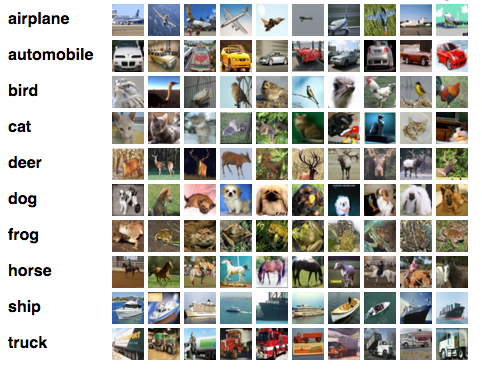
\includegraphics[width=\linewidth]{images/cifar10example.png}
  \caption{Classes of CIFAR10 including 10 random images from each \cite{CIFAR}}
  \label{fig:cifar10}
\end{figure}
Figure \ref{fig:cifar10} shows a boat.

We use CIFAR datasets as is, meaning that we also share same train/test dataset split for evaluating generated CNN architectures. There are 50000 training images and 10000 test images in the dataset.

\section{Metrics}
\section{Environment and training}
\section{Results}
